\documentclass[12pt]{report}

\usepackage[a4paper]{geometry}

%\geometry{left=2.5cm,right=2.5cm,top=2.5cm,bottom=2.5cm, a4paper}
\usepackage{multicol}
\usepackage[utf8]{inputenc}
\usepackage{amsmath}
\usepackage{amsthm}
\usepackage{amssymb}
\usepackage{ulem}
\usepackage{graphicx}
\usepackage{caption}
\graphicspath{ {./Images/} }
\usepackage[document]{ragged2e}
\usepackage{setspace}
\usepackage{tabularx}
\usepackage[slovene]{babel}
\usepackage{textcomp, gensymb}
\usepackage{siunitx}
\usepackage{pdfrender,xcolor}
\usepackage{hyperref}
\usepackage{xurl}
\usepackage{float}
\usepackage{titlesec}
\usepackage{parskip}

\newcommand{\N}{\mathbb{N}}
\newcommand{\R}{\mathbb{R}}
\newcommand{\C}{\mathbb{C}}
\newcommand{\Z}{\mathbb{Z}}



\newfloat{slika}{htbp}{loc}
\floatname{slika}{Slika}

\newfloat{tabela}{htbp}{loc}
\floatname{tabela}{Tabela}

% Differential
\newcommand{\diff}{\mathrm{d}}


\title{

  {MAT 1 ustni del}\\
  {\small Rešitve pogostih vprašanj}\\

}
\date{januar 2025}
\author{Jure Kos}


\titleformat{\chapter}[hang]{\Huge\bfseries}{\thechapter{. }}{0pt}{\Huge\bfseries}

\setlength\parindent{0pt}

\begin{document}


\maketitle

\chapter*{Številske množice}

\section*{Naravna števila (lastnosti in operacije)}
So števila, s katerimi štejemo. Možne operacije so seštevanje in množenje. 1 je nevtralni element za množenje. Množica je urejena. 2 naravni števili $a$ in $b$ lahko primerjamo. Lahko velja $a<b$ ali $a>b$ ali $a=b$. Vsakemu naravnemu številu lahko določimo neposrednega naslednika in tudi neposrednega predhodnika izjema je število $1$. V množici naravnih števil je naslednik $n+1$ predhodnik pa $n-1$. Vsaka podmnožica naravnih števil ima najmanjši element. Je števno neskončna.

\section*{Matematična indukcija}
Pri indukciji pokažemo, da neka lastnost velja za vsa naravna števila. Za indukcijo potrebujemo bazo indukcije in indukcijski korak.\\
\bigbreak
Baza indukcije: dokažemo, da lastnost velja za najmanjše naravno število (število $1$).\\
\bigbreak
Indukcijski korak: dokažemo, da velja za vsa naslednja naravna števila, tako da predpostavimo, da velja za $n$ in preverimo, če velja za $n+1$.

\section*{Cela števila (lastnosti in operacije)}
Množica celih števil množici naravnih doda $0$ in negativna števila. Možne operacije so seštevanje, množenje in odštevanje. $0$ je nevtralni element za seštevanje in odštevanje. So urejena množica. Vsem se da določiti neposrednega predhodnika in naslednika. Vsem podmnožicam se ne da določiti najmanjšega elementa zato izgubimo indukcijo. Je števno neskončna. Za vsako celo število $a$ je definirano nasprotno število $-a$ za katerega velja $a+(-a)=0$. Število $-a$ je inverzni element za seštevanje.
		
\section*{Racionalna števila (lastnosti in operacije)}
Množica racionalnih števil je množica vseh števil, ki jih lahko zapišemo z ulomkom $\frac{a}{b}$, kjer sta $a$ in $b$ celi števili in $b$ ni $0$. Množica je urejena in števno neskončna. Številom ni možno določiti predhodnika ali naslednika. Dokaz za to: če imaš 2 racionalni števili $\frac{a}{b}$ in $\frac{c}{d}$, jima lahko določiš aritmetično sredino po formuli $\frac{\frac{a}{b}+\frac{c}{d}}{2}$. Nastalo racionalno število leži med originalnima številoma. Definirane so operacije $+ - \cdot$ in $/$. 


\section*{Iracionalna števila ($\sqrt{2},\pi,e, ...$)}
So števila, ki se jih ne da zapisati z ulomkom. V decimalni obliki imajo neskončen neperiodičen zapis.

\section*{Realna števila (lastnosti in operacije)}
Realna števila so unija racionalnih in iracionalnih števil. Množica je neštevno neskončna. Množica je urejena. Množica racionalnih števil je gosta v množici realnih števil (za vsako realno število obstaja za poljubno majhen $\varepsilon$ na intervalu ($r-\varepsilon$, $r+\varepsilon$) racionalno število). V množici realnih števil so definirane operacije $+ - \cdot$ in $/$.

\section*{Decimalni zapis realnega števila}
Decimalni zapis spravi število na potence števila $10$.\\ 
Primer: $126,83 = 1 \cdot 10^{2} + 2 \cdot 10^{1} + 6 \cdot 10^{0} + 8 \cdot 10^{-1} + 3 \cdot 10^{-2}$. \\
Celi del od decimalnega ločuje decimalna vejica.

\section*{Absolutna vrednost}
Predstavlja oddaljenost števila od izhodišča številske premice. Pri pozitivnih vrednostih je absolutna vrednost enaka originalnemu številu, pri negativnih se predznak obrne na pozitiven. Oznaka absolutne vrednosti števila $a$ je $|a|$. Lastnosti: $|a\cdot b|=|a|\cdot|b|$, $|-a|=|a|$, $|a+b| \leq |a|+|b|$.

\section*{Kompleksna števila (lastnosti in operacije)}
Enačbe $x^{2}=-1$ se v realnih številih ne da rešiti. Rešitev te enačbe je število $i$. Kompleksna števila so sestavljene iz realnega in imaginarnega dela. Zapisujejo se v obliki $a+bi$. $a$ predstavlja realno komponento $b$ pa imaginarno. $i$ ni del imaginarne komponente. Če je realna komponenta $0$ in imaginarna ni $0$ tedaj je število v celoti imaginarno. Definirane operacije za kompleksna števila so $+ - \cdot /$ in konjugiranje, ki imaginarni komponenti obrne predznak.

\section*{Polarni zapis kompleksnega števila}
Kompleksna števila se prikazuje v kompleksni ravnini. Točke v ravnini se lahko poda s koordinatama ali s polarnim kotom in radijem. Radij kompleksnega števila je njegova absolutna vrednost, ki se jo dobi po formuli $\sqrt{a^{2}+b^{2}}$. Polarni kot se dobi preko kotnih funkcij. $\frac{b}{a} = \tan\varphi$, torej je $\varphi=\arctan(\frac{b}{a})$. Pri iskanju kota je potrebno biti pozoren na kvadrant v katerem se kompleksno število nahaja. arctg vrne vrednosti med $0$ in $\pi$, zato je potrebno vrednostim v 3. in 4. kvadrantu prišteti $\pi$. Polarni zapis je oblike $r(\cos\varphi + i\cdot \sin\varphi)$. Za pretvarjanje iz polarnega zapisa v kartezični ponovno uporabimo kotne funkcije po formulah $a=r\cdot \cos\varphi, b=r \cdot \sin\varphi$

\section*{De Moivrova formula}
De Moivrova formula se uporablja za hitro potenciranje kompleksnega števila. Število mora biti v polarni obliki. Tedaj velja 
\[(r(\cos\varphi + i \cdot \sin\varphi))^{n}=(r^{n})(\cos(n\varphi) + i \cdot \sin(n\varphi))\]. 
\bigbreak
Pri korenjenju n-te stopnje gre $r$ pod koren n-te stopnje in $\varphi$ se deli z $n$ (eksponent $\frac{1}{n}$ po zgornji formuli). Dobimo $n$ rešitev na krožnici z enakimi razmaki.\\
\bigbreak
Primer: \[(16(\cos\pi + i \sin\pi))^{\frac{1}{4}} = 16^{\frac{1}{4}}(\cos(\frac{\pi}{4}) + i\sin(\frac{\pi}{4})) =  2(\cos(\frac{\pi}{4})+i\sin(\frac{\pi}{4}))\].\\ 
\bigbreak
To je samo ena rešitev, ker imajo rešitve med seboj enake razmake prištejemo osnovni rešitvi $k\frac{2\pi}{n}$, kjer je k celo število med 0 in vključno $n-1$. Na istem primeru je $\frac{2\pi}{n}=\frac{\pi}{2}$ in vrednosti $k = {0, 1, 2, 3}$. Vse rešitve enačbe so tako:

\[2(\cos(\frac{\pi}{4}+0))+i\sin(\frac{\pi}{4}+0))\]
\[2(\cos(\frac{\pi}{4}+\frac{\pi}{2})+i\sin(\frac{\pi}{4}+\frac{\pi}{2}))\]
\[2(\cos(\frac{\pi}{4}+\frac{2\pi}{2})+i\sin(\frac{\pi}{4}+\frac{2\pi}{2}))\]
\[2(\cos(\frac{\pi}{4}+\frac{3\pi}{2})+i\sin(\frac{\pi}{4}+\frac{3\pi}{2}))\]

ali v poenostavljeni obliki

\[2(\cos(\frac{\pi}{4})+i\sin(\frac{\pi}{4}))\]
\[2(\cos(\frac{3\pi}{4})+i\sin(\frac{3\pi}{4}))\]
\[2(\cos(\frac{5\pi}{4})+i\sin(\frac{5\pi}{4}))\]
\[2(\cos(\frac{7\pi}{4})+i\sin(\frac{7\pi}{4}))\]





\chapter*{Zaporedja}

\section*{Zaporedja in lastnosti zaporedij}
Zaporedje realnih števil je predpis, ki vsakemu naravnemu številu priredi realno število. Pišemo ga kot ${a_n}, n \in \N$, kjer je $a_n$ n-ti člen zaporedja. Zaporedje lahko podamo z eksplicitnim zapisom ($a_n$ je odvisen od $n$) ali z rekurzivnim zapisom ($a_n$ je podan s prejšnjimi členi, hkrati moramo podati še nekaj začetnih členov). Predstavimo ga lahko z grafom v ravnini $\R^2$ ali kot točke na številski premici.\\
\bigbreak
Zaporedje je aritmetično, če je razlika (diferenca $[d]$) sosednjih dveh členov konstantna.\\
\bigbreak
Zaporedje je geometrijsko, če je kvocient $[q]$ dveh zaporednih členov konstanten.\\
\bigbreak
Zaporedje je alternirajoče, če se členom zaporedja izmenično spreminja predznak.\\
\bigbreak
Zaporedje je naraščajoče, če je $a_{n+1} \geq a_n$ za vsak $n\in \N$.\\ 
Zaporedje je strogo naraščajoče, če je $a_{n+1} > a_n$ za vsak $n\in \N$. \\
Če so vsi členi zaporedja pozitivni, bo zaporedje naraščajoče, če je kvocient dveh sosednjih členov večji (ali enak) 1. Vedno velja, da je razlika dveh sosednjih členov večja (ali enaka) 0.\\
\bigbreak
Zaporedje je padajoče, če je $a_{n+1} \leq a_n$ za vsak $n\in \N$.\\
Zaporedje je strogo padajoče, če je $a_{n+1} < a_n$ za vsak $n\in \N$.\\
\bigbreak
Zaporedje je monotono, če je bodisi naraščajoče ali pa padajoče.

\section*{Zgornje in spodnje meje zaporedij}
Zaporedje je navzgor omejeno, če obstaja $M \in \R$, da je $a_{n} \leq M$ za vsak $n\in \N$. ($M$ je tako število, da so vsi členi zaporedja manjši.) $M$ je zgornja meja zaporedja.\\

Zaporedje je navzdol omejeno, če obstaja $m \in \R$, da je $a_{n} \geq m$ za vsak $n\in \N$. ($m$ je tako število, da so vsi členi zaporedja večji.) $m$ je spodnja meja zaporedja.\\
\bigbreak
Zaporedje je omejeno, če je omejeno navzgor in navzdol.
Supremum je najmanjša zgornja meja zaporedja (natančna zgornja meja). Število $M_0$ je supremum, če velja: $a_n \leq M_0$ in za vsak (še tako majhen) $\varepsilon > 0$ obstaja $n_0$, da je $a_{n_0} > M_0 - \varepsilon$. \\
\bigbreak
Infimum je največja spodnja meja zaporedja (natančna spodnja meja). Število $m_0$ je infimum, če velja: $a_n \geq m_0$ in za vsak (še tako majhen) $\varepsilon > 0$ obstaja $n_0$, da je $a_{n_0} < m_0 + \varepsilon$.\\
\bigbreak
Supremum in infimum sta lahko člena zaporedja (npr. pri strogo padajočem zaporedju je supremum $a_1$, pri strogo naraščajočem je infimum $a_1$). 

\section*{Limite in stekališča zaporedij}
Število $A$ je stekališče zaporedja, če za vsak $\varepsilon > 0$ obstaja neskončno mnogo členov zaporedja, za katere velja $|A - a_n| < \varepsilon$.\\
\bigbreak
Število $A$ je limita zaporedja, če za vsak $\varepsilon > 0$ obstaja $n\in \N$, da je $|A - a_n| < \varepsilon$ za vsak $n > n_0$ (od nekega $n$ dalje vsi členi ležijo v $\varepsilon$ okolici števila $A$).\\
\bigbreak
Izven $\varepsilon$ okolice leži le končno mnogo členov.
Vsaka limita je stekališče, ni pa vsako stekališče limita. 

\section*{Konvergenca zaporedij in Cauchyjev pogoj}
Če limita zaporedja obstaja, potem je to zaporedje konvergentno.\\
Če limite ni, je divergentno.\\
\bigbreak

Če je zaporedje naraščajoče in navzgor omejeno, potem je konvergentno - limita je enaka supremumu. \\
Če je zaporedje padajoče in navzdol omejeno, je konvergentno - limita je enaka infimumu.\\
\bigbreak
Cauchyjev pogoj: Zaporedje je konvergentno natanko tedaj, ko za vsak $\varepsilon > 0$ obstaja $n\in \N$, tako da za vse $n > n_0$ in vse $k \in \N$ velja $|a_n - a_{n+k}| < \varepsilon$ (za vsak $\varepsilon > 0$ od nekega člena $a_{n_0}$ naprej se poljubna dva člena zaporedja razlikujeta za manj kot $\varepsilon$). 

\section*{Limita zaporedja $a_n=c^n, c \in \R$}

 \[\lim_{n \to \infty}C^n= \begin{Bmatrix}
  \nexists; c\leq-1 \\
  0; |c| < 1 \\
  1; c = 1 \\
  \infty; c > 1 \\
 \end{Bmatrix}\]

\section*{Definicija potence z iracionalnim eksponentom}
Radi bi definirali $c^r$, kjer je $r, c \in \R, c > 0$.
Izberemo zaporedje ${q_n}$ racionalnih števil, ki konvergira proti r:
\[\lim_{n \to \infty} q_n = r\].

Ker je ${q_n}$ konvergentno, ustreza Cauchyjevemu pogoju, zato tudi ${c^{q_n}}$ ustreza Cauchyjevemu pogoju, torej tudi to zaporedje konvergira.
\[c^r = \lim_{n \to \infty} c^{q_n}\] - limita je neodvisna od izbire zaporedja $q_n$.

\section*{Definicija števila e}
$e$ ali Eulerjevo število je osnova naravnega logaritma. Funkcija $e^x$ je edina funkcija, za katero velja $f’(x)=f(x)$. Je iracionalen, njegova vrednost je približno $2,718$. Dobi se ga po formuli
\[e=\lim_{n \to \infty}(1+\frac{1}{n})^n\]
 



\chapter*{Številske vrste}

\section*{Številske vrste}
Vsoto neskončno členov zaporedja imenujemo številska vrsta. Označi se jo kot

\[\sum_{n=1}^{\infty}a_n\]
 
$a_n$ se imenuje splošni člen vrste. Če seštejemo končno število členov se to imenuje delna vsota in se označuje s $s_n$.

\section*{Delne vsote in konvergenca vrst}
Vrsta je konvergentna, če je njena vsota enaka končni vrednosti. Za konvergenco mora konvergirati zaporedje delnih vsot.

\[s_n=\sum_{i=1}^{n}a_i\]

Da vrsta konvergira, mora zaporedje $a_n$ imeti limito v neskončnosti enako 0. Če limita zaporedja ni enaka 0, vrsta vedno divergira.

\section*{Cauchyjev pogoj za vrste}
Če je vrsta konvergentna za vsak $\varepsilon>0$, obstaja naravno število $n_0$ za katerega velja 
 \[\varepsilon > \sum_{n=n_0}^{\infty}a_n\]

\section*{Geometrijska vrsta}
Je vrsta za katero velja $ \frac{a_{n+1}}{a_n}=q$, kjer je $q$ konstanten za vse $n$. Geometrijska vrsta konvergira kadar velja $-1<q<1$

\section*{Harmonična vrsta}
 
 \[\sum_{n=1}^{\infty}\frac{1}{n}\]
Vrsta členov zaporedja $\frac{1}{n}$ se imenuje harmonična vrsta. Limita zaporedja je sicer enaka 0, vrsta pa divergira.

\section*{Kriteriji za konvergenco vrst}
\emph{Kvocientni kriterij}: Velja za vrste s pozitivnimi členi. Pri kvocientnem kriteriju gledamo limito kvocienta zaporednih členov v neskončnosti. Vrednost limite označimo s $q$.
 
 \[q = \lim_{n \to \infty}\frac{a_n+1}{a_n}\]
 
Če je $q < 1$, vrsta konvergira, če je $q > 1$, vrsta divergira in če je $q=1$, kriterij odpove.

\emph{Korenski kriterij}: Pri korenskemu kriteriju gledamo limito n-tega korena $a_n$ ko pošljemo $n$ v neskončnost. Vrednost limite označimo s $q$.
 
 \[q = \lim_{n \to \infty}\sqrt[n]{a_n}\]
 
Če je $q < 1$, vrsta konvergira, če je $q > 1$, vrsta divergira in če je $q=1$, kriterij odpove.

\emph{Primerjalni kriterij}: Če imamo dve vrsti $\displaystyle\sum_{n=1}^{\infty}a_n$ in $\displaystyle\sum_{n=1}^{\infty}b_n$ in za vsak $n$ velja $0<a_n<b_n$:
Če vrsta $\displaystyle\sum_{n=1}^{\infty}b_n$ konvergira, tedaj tudi vrsta $\displaystyle\sum_{n=1}^{\infty}a_n$ konvergira.

Če vrsta $\displaystyle\sum_{n=1}^{\infty}a_n$ divergira, tedaj tudi vrsta $\displaystyle\sum_{n=1}^{\infty}b_n$ divergira

Bonus kriterij za vrste z racionalnimi predpisi: Če je predpis zaporedja racionalna funkcija in je stopnja imenovalca od stopnje števca večja za 2 ali več, vrsta konvergira.

\section*{Alternirajoče vrste in Leibnitzov kriterij}
Vrsta  $\displaystyle\sum_{n=1}^{\infty}a_n$ je alternirajoča, ko velja $a_n \cdot a_{n+1}<0$ za vsak $n$. Leibnitzov kriterij določa konvergenco alternirajočih vrst. Če je zaporedje $|a_n|$ padajoče in velja
 \[\lim_{n \to \infty}|a_n|=0\]
tedaj alternirajoča vrsta konvergira.

\section*{Absolutna konvergenca vrste}
Vrsta $\displaystyle\sum_{n=1}^{\infty}a_n$ absolutno konvergira, če konvergira vrsta  $\displaystyle\sum_{n=1}^{\infty}|a_n|$ . Vsaka absolutno konvergentna vrsta je konvergentna.

 


\chapter*{Funkcije}

\section*{Definicija preslikave in funkcije}
Preslikava je predpis, ki vsakemu elementu $a$ iz množice $ \mathcal{A}$ priredi natanko določen element $f(a)$ iz množice $ \mathcal{B}$. $f(a$) je slika elementa $a$. 
Funkcija je vrsta preslikave, ki slika iz neke podmnožice realnih števil v realna števila.

\section*{Definicijsko območje in zaloga vrednosti preslikave}
Množica $ \mathcal{A}$ je definicijsko območje, množica $ \mathcal{B}$ je kodomena.
Množica vseh slik se imenuje zaloga vrednosti in je podmnožica kodomene.

\section*{Injektivne, surjektivne in bijektivne funkcije}
Preslikava je injektivna, če je vsak element iz $ \mathcal{B}$ slika kvečjemu enega elementa iz $ \mathcal{A}$. \\
\bigbreak
Preslikava je surjektivna, če je vsak element iz $ \mathcal{B}$ slika vsaj enega elementa iz $ \mathcal{A}$. \\
\bigbreak
Preslikava je bijektivna, če je vsak element iz $ \mathcal{B}$ slika natanko enega elementa iz $ \mathcal{A}$ - preslikava je hkrati injektivna in surjektivna.

\section*{Kompozitum preslikav}
Naj bodo $ \mathcal{A}$, $ \mathcal{B}$ in $ \mathcal{C}$ neprazne množice, določimo preslikavi $f: \mathcal{A} \to \mathcal{B}$ in $g: \mathcal{B} \to \mathcal{C}$. Kompozitum preslikav definiramo kot $f \circ g: \mathcal{A} \to \mathcal{C}$, $(f \circ g)(a) = f(g(a))$.

\section*{Lihe in sode funkcije}
Funkcija je liha, če velja $f(-x) = -f(x)$. Graf takšne funkcije je simetričen glede na izhodišče.\\
\bigbreak
Funkcija je soda, če velja $f(-x) = f(x)$. Graf je simetričen glede na ordinatno os.

\section*{Inverzna funkcija}
Naj bo funkcija $f$ injektivna. Funkcijo $f^{-1}$, za katero velja $f^{-1}(f(x)) = x$, imenujemo inverzna funkcija. Graf takšne funkcije je zrcalen grafu originalne funkcije čez simetralo lihih kvadrantov.

\section*{Polinomi in racionalne funkcije}
Polinom je funkcija oblike $f(x)= k_nx^n+k_{n-1}x^{n-1}+k_{n-2}x^{n-2}+ ... +k_1x+k_0$ , kjer $k_n$ ni enak 0 in je $k_i$ realno število. $n$ je stopnja polinoma. Definicijsko območje vsakega polinoma so vsa realna števila. Ničle polinoma so vrednosti $x_i$ za katere velja $f(x_i)=0$. Polinom n-te stopnje ima največ $n$ realnih ničel. Polinomi lihih stopenj imajo vsaj eno realno ničlo.\\
\bigbreak
Racionalna funkcija je funkcija oblike $\frac{p(x)}{q(x)}$, pri čemer sta $p$ in $q$ (neničelna) polinoma. Definicijsko območje funkcije je enako $\R$ \textbackslash $\{x; q(x) = 0\}$.
\bigbreak
Ničle racionalne funkcije so enake ničlam polinoma $p$, poli pa ničlam polinoma $q$.  Za pole velja: če so lihe stopnje, funkcija spremeni predznak, če so sode, pa ne.\\ Asimptota funkcije je taka krivulja, da se ji graf funkcije $f$ približuje, ko gre $x$ proti $\pm \infty$. Izračunamo tako, da delimo $p(x)$ z $q(x)$ - če je stopnja $p$ manjša od stopnje $q$, potem je asimptota enaka $y = 0$.\\
Če sta stopnji $p$ in $q$ enaki, je asimptota vodoravna. Graf lahko seka asimptoto (ko je ostanek pri deljenju $r(x)$ enak 0).

\section*{Eksponentna in logaritemska funkcija}
Eksponentna funkcija je podana v obliki $f(x) = a^x$. $a>0$ in $a\neq 1$. Navzgor je neomejena, navzdol pa je omejena z 0. Če je $a > 1$ potem ima funkcija limito v $-\infty$ enako 0. Ko gre $x$ proti $\infty$ pa nima limite (je neomejena). Ravno obratno velja če je $0 < a <1$.\\
$D_f = \R$ \\
$Z_f =(0,\infty)$
\bigbreak

Logaritemska funkcija je podana v obliki $f(x)=log_a(x)$. Je inverz eksponentne funkcije. Če je $a > 1$ potem funkcija povsod narašča. Če je manjši pa pada.  Logaritemska funkcija ni omejena.\\
$D_f = (0,\infty)$	\\
$Z_f = \R$

\section*{Kotne funkcije in ciklometrične funkcije}
 
\begin{slika}[H]
  \centering
  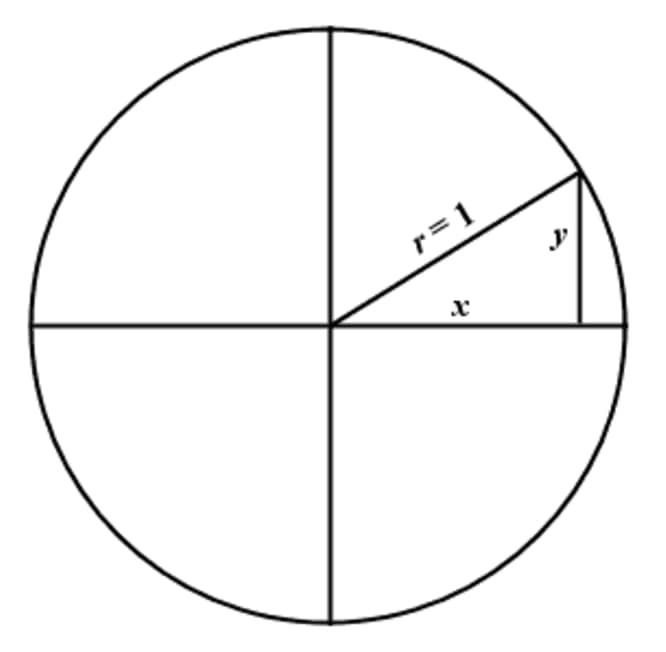
\includegraphics[width = 7cm]{18}
\end{slika}

Kotne funkcije definiramo preko enotske krožnice (krožnica z radijem 1 s središčem v koordinatnem izhodišču). Od središča krožnice na poljubno točko $T(x, y)$ na krožnici potegnemo daljico $r$. Kot $\varphi$ je definiran kot kot med abscisno osjo in $r$. Velja: $x=\cos\varphi$, $y=\sin\varphi$ $\frac{y}{x}=\tan\varphi=\frac{\sin\varphi}{\cos\varphi}$

 \begin{slika}[H]
  \centering
  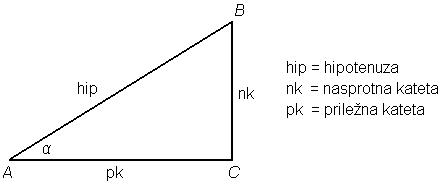
\includegraphics[width = \textwidth]{19}
\end{slika}

$x, y$ in $r$ v enotski krožnici, ko je $T$ v 1. kvadrantu, tvorijo pravokotni trikotnik. Preko podobnih trikotnikov za poljubni pravokotni trikotnik dobimo sledeče zveze: $\frac{nk}{hip} = \sin\alpha$, $\frac{pk}{hip} = \cos\alpha$, $\frac{nk}{pk} = \tan\alpha$
\bigbreak
Kotne funkcije so periodične. Sinus in kosinus imata periodo $2\pi$, tangens pa $\pi$. Sinus ima ničle v $k\pi;k\in \Z$. Kosinus ima ničle v $\frac{\pi}{2}+k\pi; k\in \Z$. Ker je tangens definiran kot $\frac{\sin}{\cos}$ ima ničle v $k\pi; k\in Z$(ničle sinusa) in pole v $\frac{\pi}{2}+k\pi; k\in \Z$(ničle kosinusa). Sinus in kosinus imata zalogo vrednosti $[-1, 1]$. Definicijsko območje so vsa realna števila. Tangens ima za zalogo vrednosti vsa realna števila, definicijsko območje pa je $x\in \R$ \textbackslash $\{\frac{\pi}{2}+k\pi; k\in \Z\}$

\begin{slika}[H]
  \centering
  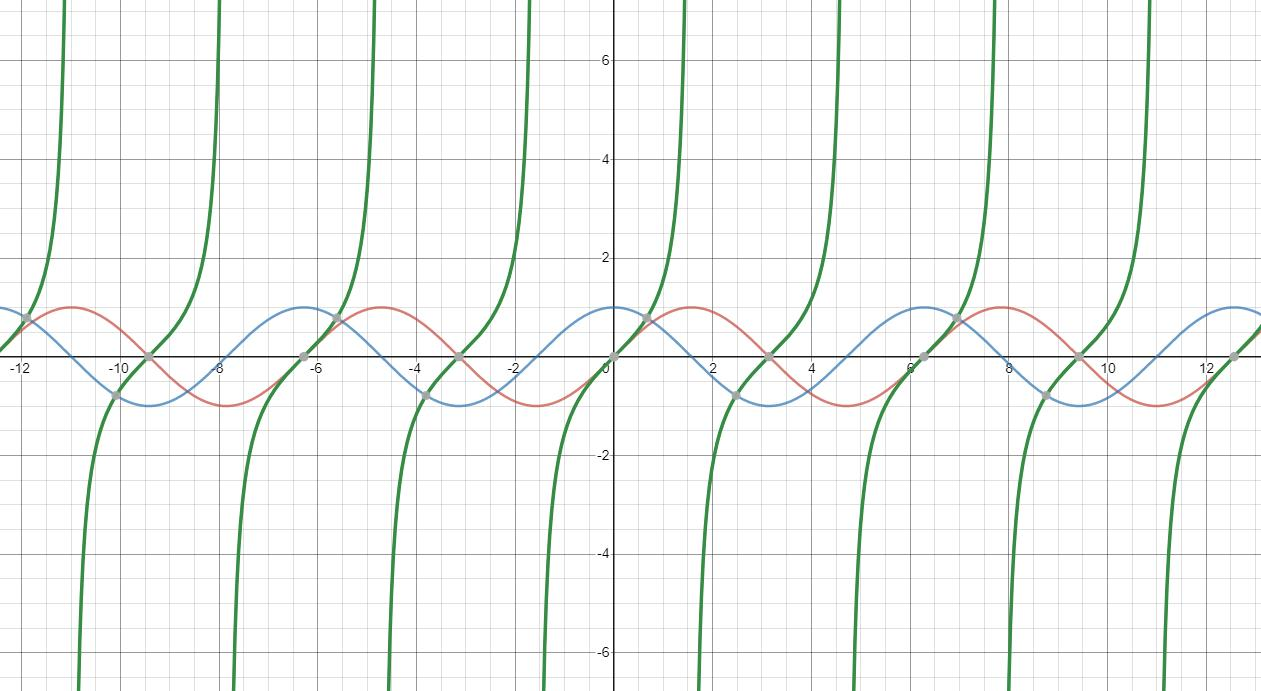
\includegraphics[width = \textwidth]{20}
\end{slika}
 
Slika prikazuje grafe $f(x)=\sin(x)$ (rdeča) $g(x)=\cos(x)$ (modra) in $h(x)=\tan(x)$ (zelena). Opazimo, da imata $\sin$ in $\cos$ enak graf, samo zamaknjen za $\frac{\pi}{2}$. Iz tega dobimo zvezo $\sin(\frac{\pi}{2}-x)=\cos(x)$ in $\cos(\frac{\pi}{2}-x)=\sin(x)$.
\bigbreak
Ciklometrične funkcije ali arkus funkcije so inverzne kotnim. Inverzno funkcijo se lahko določi samo za bijektivne funkcije, zato je potrebno kotnim funkcijam omejiti definicijsko območje. Pri $\cos$ vzamemo interval $[0, \pi]$, pri $\sin [-\frac{\pi}{2}, \frac{\pi}{2}]$ in pri $\tan  (-\frac{\pi}{2}, \frac{\pi}{2})$ .
\bigbreak
Funkcija $\arcsin$ je definirana na intervalu $[-1, 1]$ in ima zalogo vrednosti $[-\frac{\pi}{2}, \frac{\pi}{2}]$

Funkcija $\arccos$ je definirana na intervalu $[-1, 1]$ in ima zalogo vrednosti $[0, \pi]$

Funkcija $\arctan$ je definirana za vsa realna števila in ima zalogo vrednosti $(-\frac{\pi}{2}, \frac{\pi}{2})$
		
\begin{slika}[H]
  \centering
  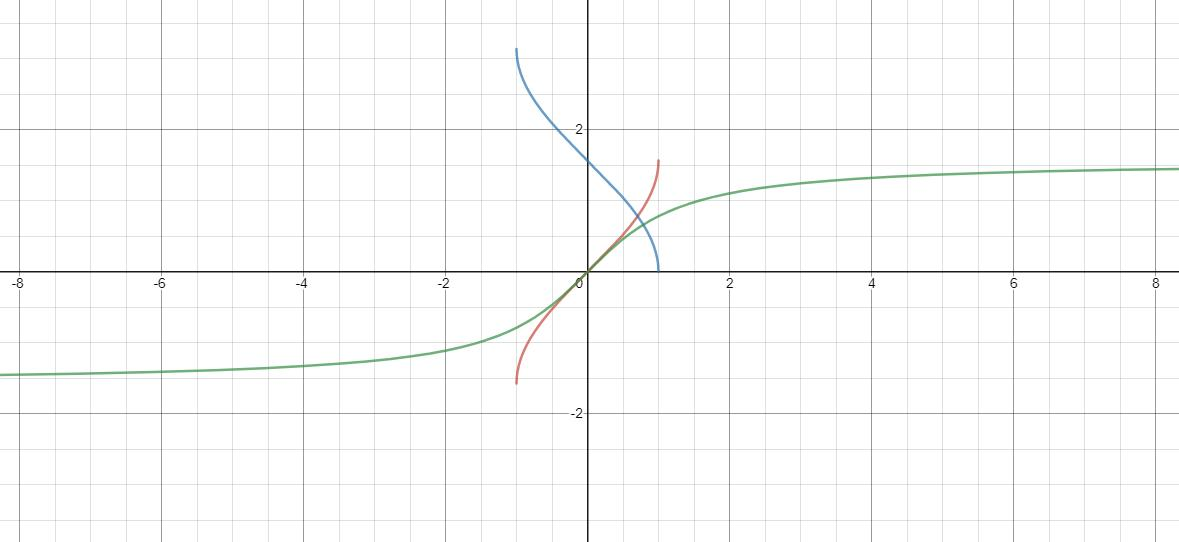
\includegraphics[width = \textwidth]{21}
\end{slika}

Slika prikazuje grafe $f(x)=\arcsin(x)$ (rdeča) $g(x)=\arccos(x)$ (modra) in$ h(x)=\arctan(x)$ (zelena). Grafa $\arcsin$ in $\arccos$ sta enaka samo zrcaljena čez $x$ os in zamaknjena za $\frac{\pi}{2}$ po $y$ osi. Iz tega dobimo zvezo 
$\arcsin(x)+\arccos(x)=\frac{\pi}{2}$

\section*{Hiperbolične funkcije in area funkcije}
Hiperbolične funkcije so podobne kotnim, le da so za hiperbole. Definirane so preko desne polovice enotske hiperbole $x^2-y^2=1$. Spet izberemo točko $T(x, y)$ na hiperboli in potegnemo daljico do izhodišča. Območje med daljico, hiperbolo in abscisno osjo predstavlja polovico hiperboličnega kota $\alpha$. Podobno velja $x=\cosh(\alpha)$, $y=\sinh(\alpha)$. 

 \begin{slika}[H]
  \centering
  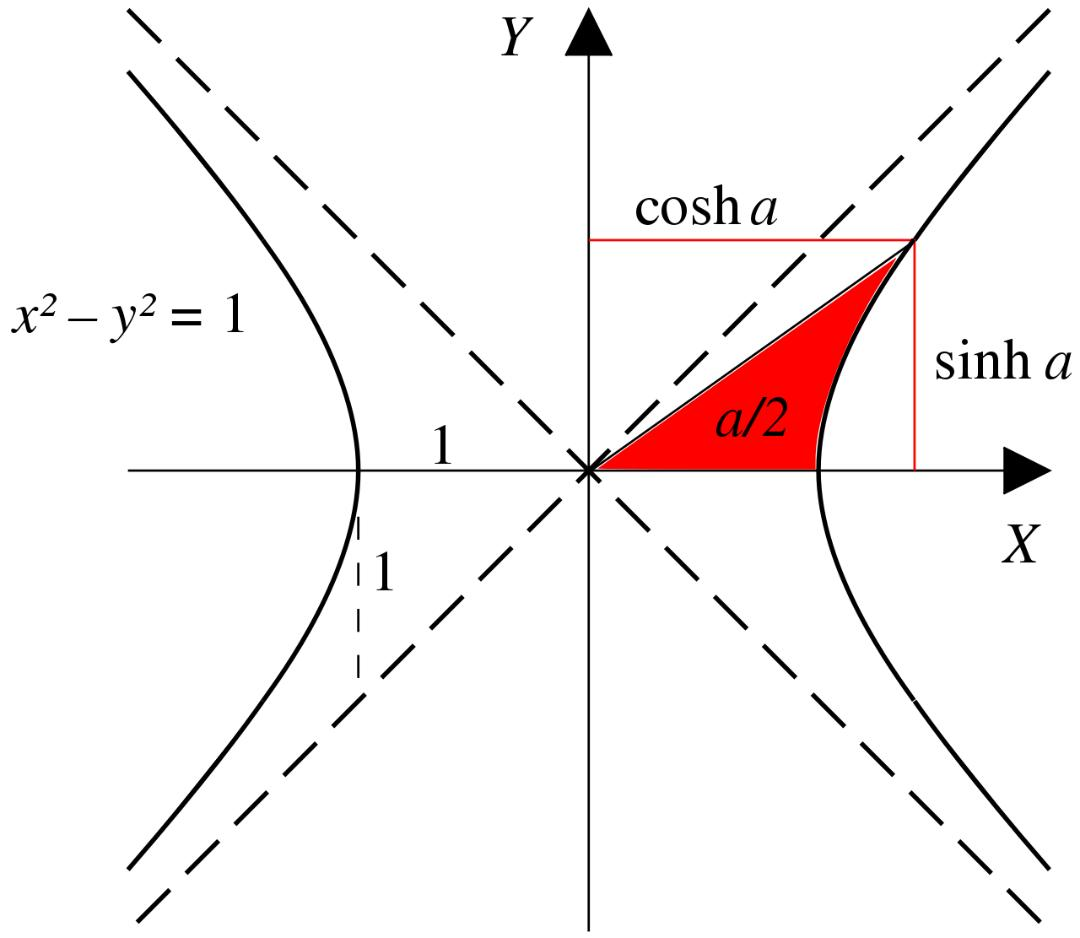
\includegraphics[width = 8cm]{22}
\end{slika}

Zapiše se jih lahko z eksponentnimi funkcijami
 
 \[\sinh x=\frac{e^x-e^{-x}}{2}\]
 \[\cosh x=\frac{e^x+e^{-x}}{2}\]
 \[\tanh x= \frac{\sinh x}{\cosh x}= \frac{e^x-e^{-x}}{e^x+e^{-x}}\]
 
  \begin{slika}[H]
  \centering
  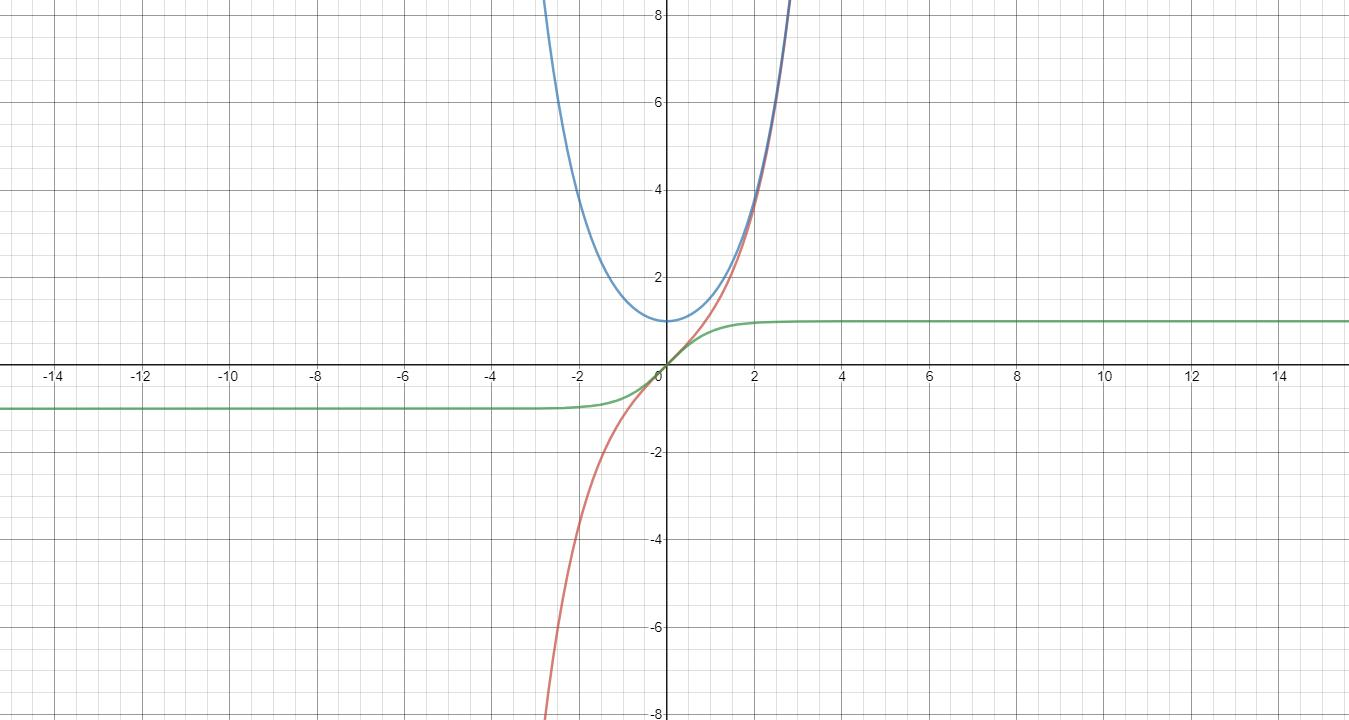
\includegraphics[width = \textwidth]{26}
\end{slika}
 
Slika prikazuje grafe $f(x)=\sinh(x)$ (rdeča), $g(x)=\cosh(x)$ (modra) in $h(x)=\tanh(x)$ (zelena).
\bigbreak
Area funkcije so inverzne hiperboličnim. Kot parameter vzamejo vrednost $x$ ali $y$ na enotski hiperboli in vrnejo hiperbolični kot. $\alpha=\operatorname{arsinh}(y)$, $\alpha=\operatorname{arcosh}(x)$
\bigbreak
Zapiše se jih lahko z logaritmi

 \[\operatorname{arsinh} x= ln(x+\sqrt{x^2+1}\]
 \[ \operatorname{arcosh}  x=ln(x+\sqrt{x^2-1}\]
 \[\operatorname{artanh} x= \frac{1}{2}ln(\frac{1+x}{1-x})\]
 


\section*{Limita funkcije, leva limita in desna limita funkcije}
Limita funkcije nam pove, kateri vrednosti se približuje $f(x_0)$, ko se $x$ približuje neki vrednosti $x_0$. Če je število $n$ limita funkcije v točki $x_0$ obstaja za vsak $\varepsilon>0$ nek $\delta>0$ za katerega velja $|f(x)-n|<\varepsilon$, ko je $|x-x_0|<\delta$ in $x\neq x_0$
\bigbreak
Limita v $x_0$ ni odvisna od vrednosti $f(x_0)$, zato jo lahko izračunamo tudi ko v $x_0$ funkcija ni definirana.
Limito $f(x)$ ko se $x$ približuje $x_0$ označujemo z  

\[\lim_{x \to x_0}f(x)\]

Leva limita funkcije poda vrednost funkcije $f(x)$, ko se približuje neki vrednosti $x$ z leve. Število $n$ je leva limita funkcije če za vsak $\varepsilon>0$ obstaja $\delta>0$ za katerega velja $|f(x)-n|<\varepsilon$ za vsak $x<x_0$ kjer je $x_0-x<\delta$
\bigbreak
Levo limito $f(x)$ označujemo z 
\[\lim_{x \uparrow x_0}f(x)\] 

Na podoben način desna limita funkcije poda vrednost funkcije $f(x)$, ko se približuje neki vrednosti $x$ z desne. Število $n$ je desna limita funkcije če za vsak $\varepsilon>0$ obstaja $\delta>0$ za katerega velja $|f(x)-n|<\varepsilon$ za vsak $x>x_0$ kjer je $x-x_0<\delta$
\bigbreak
Desno limito $f(x)$ označujemo z  
\[\lim_{x \downarrow x_0}f(x)\]

Limita funkcije obstaja samo, ko sta leva in desna limita enaki

\section*{Limita $\displaystyle \lim_{x \to 0}\frac{\sin x}{x}$}

Vrednost limite bomo izračunali s pomočjo sendvič izreka.
Če je $f(x)\leq g(x) \leq h(x)$ in je $\displaystyle \lim_{x \to x_0}f(x) = \lim_{x \to x_0}h(x) = A$ ,
 tedaj je $\displaystyle \lim_{x \to x_0}g(x)=A$
\bigbreak
Začnemo s skico enotske krožnice
 
  \begin{slika}[H]
  \centering
  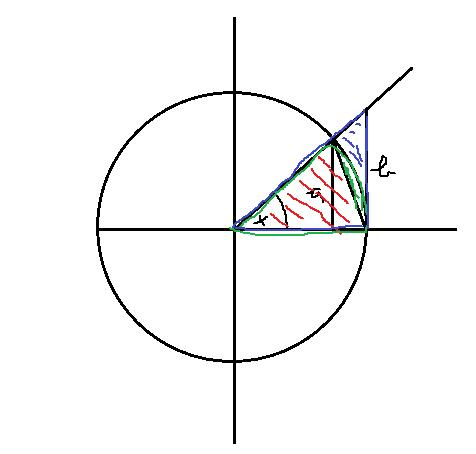
\includegraphics[width = 6cm]{37}
\end{slika} 
 
Velja: $a=\sin x$ in $b=\tan x$
Ploščino rdečega trikotnika dobimo iz osnovnice in višine $S_r=\frac{\sin x}{2}$
Ploščino modrega trikotnika dobimo iz obeh katet  $S_m=\frac{\tan x}{2}$
\bigbreak
Ploščino zelenega krožnega izseka dobimo iz ploščine kroga in kota $S_z=\frac{x\pi r^2}{2\pi}$
Velja:$S_r \leq S_z \leq S_m$ , torej je $\frac{\sin x}{2} \leq \frac{x}{2} \leq \frac{\tan x}{2}$. Enačbo množimo z 2 in delimo s $\sin x$. Dobimo $1 \leq \frac{x}{\sin x}\leq \frac{1}{\cos x}$ . Vzamemo inverzne vrednosti in dobimo $1 \geq \frac{\sin x}{x}\geq \cos x$ . Izračunamo limite 1 in $\cos x$. $\displaystyle \lim_{x \to 0}1=1$ ,. Ker velja $\displaystyle \lim_{x \to 0}\cos x=1$, $\displaystyle \lim_{x \to 0}1= \lim_{x \to 0}\cos x=1$  in $1 \geq \frac{\sin x}{x} \geq \cos x$ je po sendvič izreku  $\displaystyle\lim_{x \to 0}\frac{\sin x}{x}=1$
\bigbreak
Hitrejši način je preko L’Hospitalovega pravila, kjer lahko dobimo limito funkcije nedoločene oblike $\frac{0}{0}$ ali $\frac{\infty}{\infty}$ po formuli  \[\lim_{x \to x_0}\frac{f(x)}{g(x)}= \lim_{x \to x_0}\frac{f'(x)}{g'(x)}\]  

Torej je \[\lim_{x \to 0}\frac{\sin x}{x}= \lim_{x \to 0}\frac{\cos x}{1} = 1 \]

\section*{Zveznost funkcije}
Funkcija je zvezna ko “nima lukenj”.
Funkcija $f:D \to \R$, $D \subseteq \R$ je zvezna v točki $x_0$, če za vsak $\varepsilon>0$ obstaja tak $\delta>0$, da je $|f(x)-f(x_0)|<\varepsilon$ za vsak $x$, za katerega velja $|x-x_0|<\delta$. Funkcija je zvezna na $D$, če je zvezna za vsak $x\in D$.

\section*{Lastnosti zveznih funkcij na zaprtem intervalu}
Če je $f(a)f(b)<0$ (nasprotni predznak), tedaj je na intervalu $[a, b]$ vsaj ena ničla

Na zaprtem intervalu so zvezne funkcije omejene

Zvezna funkcija na zaprtem intervalu doseže svojo natančno zgornjo in spodnjo mejo

Zvezna funkcija na zaprtem intervalu $[a, b]$ doseže vsako vrednost med $f(a$) in $f(b)$.





\chapter*{Odvod}

\section*{Definicija odvoda funkcije in geometrijski pomen odvoda}
$\displaystyle f'(x)=\lim_{h \to 0}\frac{f(x+h)-f(x)}{h}$
Geometrijski pomen: Odvod funkcije $f$ v točki $x$ nam pove, kako hitro se vrednost funkcije $f$ v $x$ spreminja (smerni koeficient tangente na graf funkcije v 
tej točki).

Izpeljave nekaterih osnovnih odvodov

$(x^n)’$
Izračunamo po definiciji

\[(x^n)'= \lim_{h \to 0}\frac{(x+h)^n-x^n}{h}\]
 
$(x+h)^n$ razstavimo po binomskem izreku

\[(x^n)'= \lim_{h \to 0}\frac{x^n +\frac{n!}{1!(n-1)!}x^{n-1}h+...+\frac{n!}{1!(n-1)!}xh^{n-1}+h^n-x^n}{h}\]
 
$x^n$ in $-x^n$ se krajša, delimo s $h$
 
\[(x^n)'= \lim_{h \to 0}\bigl(\frac{n!}{1!(n-1)!}x^{n-1}+...+\frac{n!}{1!(n-1)!}xh^{n-2}+h^{n-1}\bigr)\] 
 
Vsi členi razen prvega postanejo 0. krajšamo z $(n-1)!$
Končni rezultat

\[(x^n)'=nx^{n-1}\]
 
Ali po drugi poti 
\[\left(x^n\right)’=e^{lnx \cdot n}n\frac{1}{x}=x^n \frac{n}{x}= nx^{n-1}\]

$(\sin(x))’$
Izračunamo po definciji
 
 \[(\sin x)'=\lim_{h \to 0}\frac{\sin(x+h)-\sin x}{h}\]
 
$\sin(x+h)$ razbijemo po adicijskem izreku

 \[(\sin x)'=\lim_{h \to 0}\frac{\sin x \cos h + \cos x \sin h -\sin x}{h}\]
 
Razstavimo na dve limiti
 
 \[(\sin x)'=\lim_{h \to 0}\frac{\cos x \sin h}{h} + \lim_{h \to 0}\frac{\sin x \cos h -\sin x}{h}\]
 
Iz leve limite izpostavimo $\cos x$, iz desne pa $-\sin(x$).
 
 \[(\sin x)'=\lim_{h \to 0}\cos x \frac{\sin h}{h} - \lim_{h \to 0}\sin x\frac{1- \cos h}{h}\]
 
Limita $\frac{\sin h}{h}$ ko gre $h$ proti 0 gre v 1, limita od $\frac{1- \cos h}{h}$ ko gre $h$ proti 0 gre v 0. Ostane

 
 \[(\sin x)'=1\cos x - 0\sin x= \cos x\]
 

\section*{Tangente in normala na graf funkcije}
Izračunamo 1. odvod funkcije in vstavimo tisti $x$ kjer nas zanima tangenta rezultat je koeficient tangente. V enačbo $y = kx+n$ vstavimo točko in tako dobimo enačbo tangente.
Pri normali moramo vedeti da je $k_t \cdot k_n = -1$

\section*{Pravila za odvajanje}


\begin{tabela}[H]
  \centering
  \[
      \begin{array}{|c|c|} \hline
      f(x)&f'(x)\\ \hline 
    C &   0 \\
	f(x) \pm g(x) &   f'(x) \pm g'(x) \\
	C \cdot f(x) &  C \cdot f'(x)  \\
	f(x) \cdot g(x) & f'(x)\cdot g(x) +  f(x)\cdot g'(x)  \\
	\frac{f(x)}{g(x)} &  \frac{f'(x)\cdot g(x) -  f(x)\cdot g'(x)}{(g(x))^2}  \\
	(f \circ g)(x) &   f'(g(x)) \cdot g'(x)  \\ \hline
    \end{array}
  \]
\end{tabela}

\section*{Odvod inverzne funkcije}

\[(f^{-1}(x))'=\frac{1}{f'(f^{-1}(x))}\]
 
\section*{Diferencial funkcije in računanje približnih vrednosti funkcije}
 
\[\eta=\frac{f(x+h)-f(x)}{h}-f'(x)\] 
 
Ko se $h$ približuje 0 se $\eta$ približuje 0. Pomnožimo enačbo s $h$ in damo $f’(x)$ na drugo stran.

\[f(x+h)-f(x)=\eta h + f'(x)h\] 
 
$f(x+h)-f(x)$ predstavlja spremembo vrednosti funkcije in jo označimo z $\Delta f$. $h$ predstavlja spremembo spremenljivke $x$. Označimo ga z $\Delta x$. Dobimo končno enačbo

\[\Delta f = f'(x)\Delta x+ \eta \Delta x\]
 
$f’(x)\Delta x$ se imenuje diferencial funkcije in ga označimo z $df$. $\eta$ je razlika med dejansko spremembo funkcije in diferencialom funkcije. Za majhne $\Delta x$ postane $\eta$ v primerjavi z $df$ majhen, zato ga lahko zanemarimo in s pomočjo diferencialov računamo približne vrednosti funkcije. Pri računanju približne vrednosti $f(x_0$) vzamemo funkcijo v vrednosti $x$ ki jo znamo izračunati. $x$ mora biti blizu $x_0$, da dobimo dober približek. $h$ je v tem primeru $x_0-x$. Vstavimo v enačbo

\[f(x+h) \doteq f(x)+f'(x)h\]
 

\section*{Višji odvodi funkcije}
Višje odvode dobimo, ko odvod ponovno odvajamo. Odvod odvoda se imenuje drugi odvod in se označuje z $f''(x)$. Odvod drugega odvoda se imenuje tretji odvod in se označuje z $f'''(x)$. Na podoben način se definira ostale višje odvode, se jih pa od vključno četrtega odvoda dalje označuje s številko v oklepaju. \\

Primer: 6. odvod $f(x) = f^{(6)}(x)$

\section*{Naraščanje in padanje funkcij in povezava z odvodom}
Odvod je enak naklonu tangente na graf funkcije. Ko je naklon tangente pozitiven funkcija narašča, ko je negativen funkcija pada. \\
Torej ko je $f’(x)<0$ funkcija pada,\\
 ko je $f’(x)>0$ funkcija narašča.\\
 Če je $f'(x)=0$ je tam stacionarna točka.

\section*{Fermatov izrek}
Če je $f: [a,b] \to \R$ odvedljiva funkcija, ki ima v točki $x_0$ lokalni ekstrem, tedaj je $f’(x_0) = 0$ (točka $x_0$ je stacionarna točka funkcije).

\section*{Rollov izrek}
Naj bo $f: [a,b] \to \R$ odvedljiva funkcija in naj velja $f(a) = f(b)$. Potem obstaja vsaj ena točka $x_0$, da je $f'(x_0) = 0$.

\section*{Lagrangov izrek}
Naj bo $f: [a,b] \to \R$ odvedljiva funkcija. Tedaj obstaja vsaj ena točka $x_0$, za katero velja $f'(x_0)=\frac{f(b) - f(a)}{b - a}$.\\
Kar pomeni, da na intervalu $[a,b]$ obstaja vsaj ena točka $x_0$, v kateri je naklon tangente na graf (torej odvod v tej točki) enak naklonu sekante skozi krajišči  intervala.

\section*{Stacionarne točke funkcije}
So točke, za katere velja $f'(x_0)=0; x_0 \in D_f$
Tangenta grafa v stacionarni točki je vzporedna abscisni osi

\section*{Lokalni ekstremi funkcije}

Se nahajajo v ničlah odvoda. Torej funkcijo odvajamo in ta odvod enačimo z 0.

\section*{Določanje lokalnih ekstremov s prvim in drugim odvodom funkcije}
Funkcija ima lokalni minimum v $x_0$, če obstaja tak $\delta>0$ da je $f(x_0+h)-f(x_0)>0$ za vsak $|h|<\delta$\\
Funkcija ima lokalni maksimum v $x_0$, če obstaja tak $\delta>0$ da je $f(x_0+h)-f(x_0)<0$ za vsak $|h|<\delta$\\
\bigbreak
$f'(x_0) = 0$ in $f''(x_0) < 0$: funkcija ima v $x_0$ lokalni maksimum.\\
$f'(x_0) = 0$ in $f''(x_0) > 0$: funkcija ima v $x_0$ lokalni minimum.\\
$f'(x_0) = 0$ in $f''(x_0) = 0$: funkcija ima v $x_0$ prevoj\\

\section*{Prevoji, konveksnost in konkavnost funkcije}

Funkcija je na intervalu $[a,b]$ konveksna, če sekanta skozi graf funkcije v točkah $f(a)$ in $f(b)$ leži nad grafom funkcije. Če leži pod grafom pa je konkavna.\\
Prevoj je točka na grafu v kateri funkcija preide iz konkavnosti v konveksnost ali obratno.
\bigbreak


2. odvod nam pove ali je funkcija konkavna/konveksna in hkrati kako se spreminja vrednost 1. odvoda
\bigbreak

$f''(x) > 0$: funkcija je konveksna.\\
$f''(x) < 0$: funkcija je konkavna.\\
$f''(x) = 0$: funkcija ima prevoj.

\section*{Globalni ekstremi funkcije na danem območju}
Globalni maksimum funkcije na intervalu $[a,b]$ je največja vrednost funkcije na intervalu $[a,b]$.
Ekstremi so možni na točkah, kjer je odvod funkcije enak nič, na mejah intervala $[a, b]$ ter v točkah, kjer funkcija ni odvedljiva. To najlažje preverimo tako, da $x$ vstavimo v funkcijo. Lahko pa tudi tako:
\bigbreak
$f'(x) = 0$ in $f''(x) < 0$: funkcija ima tu lokalni maksimum.\\
$f'(x) = 0$ in $f''(x) > 0$: funkcija ima tu lokalni minimum.\\
Preverjamo kateri $y=f'(x)$ je večji/manjši za globalni maksimum/minimum.

\section*{L’Hospitalovo pravilo}
Ko pri računanju limite pridemo do funkcije nedoločene oblike $\frac{0}{0}$ ali $\frac{\infty}{\infty}$ lahko limito izračunamo tako, da števec in imenovalec odvajamo.
 
Odvajamo lahko tolikokrat, dokler imamo funkcijo prej omenjene nedoločene oblike






\chapter*{Nedoločeni integral}

\section*{Nedoločeni integral}
Je družina funkcij $F(x$) katerih odvod je enak funkciji $f(x)$. Takim funkcijam $F$ pravimo primitivne funkcije.
$\int f(x)dx=F(x)+C$,	pri čemer je $F'(x)=f(x$)

\section*{Nedoločeni integrali elementarnih funkcij}
\begin{multicols}{2}
\[\int x^ndx=\frac{x^{n+1}}{n+1}+C\]
\[\int \frac{1}{x}dx=ln\ x+C\]	
\[\int e^xdx=e^x+C\]
\[\int a^xdx=\frac{1}{ln\ a}{\ a}^x+C\]
\[\int sin\ x\ dx=\ -cos\ x+C\]
\columnbreak
\[\int cos\ x\ dx=sin\ x+C\]
\[\int \frac{1}{{(cos\ x)}^2}dx=tan\ x+C\]
\[\int \frac{1}{\sqrt{1-x^2}}dx=arcsin\ x+C\]
\[\int \frac{1}{1+x^2}dx=arctan\ x\ +C\]
\[\int \frac{1}{\sqrt{1+x^2}}dx=log(x+\sqrt{1+x^2})+C\]
\end{multicols}

	


\section*{Pravila za integriranje}
\[ \int (f(x)\pm g(x))\ dx=\int f(x)\ dx\pm\int g(x)\ dx\]
\[\int k\cdot f(x)\ dx=k\cdot\int f(x)\ dx\]

\section*{Vpeljava nove spremenljivke v integral}
\[\int f(x)dx=\int f(x(t))x'(t)dt\]

\section*{Integracija po delih (per-partes)}
\[\int u(x)\cdot v'(x)\cdot dx=u(x)\cdot v(x)-\int u'(x)\cdot v(x)\cdot dx\]

ali krajše

\[\int udv=u v-\int v du\]

\section*{Integral racionalne funkcije}
\[\int \frac{p(x)}{q(x)}dx=\int\left(k(x)+\frac{r(x)}{q(x)}\right)dx\]

\section*{Integrali s trigonometričnimi funkcijami}
Naj bo $R$ racionalna funkcija sinusov in kosinusov, torej v števcu in imenovalcu nastopata polinoma sinusov in kosinusov (npr.$\frac{\sin 2x \cos x-4 \cos x}{3\cos 4x -\sin x \cos x +1}$). Potem znamo integral  $\int R(\sin x, \cos x)dx$ z univerzalno substitucijo $\tan(\frac{x}{2})$ pretvoriti v integral racionalne funkcije, ki se ga da vedno rešiti.\\
\bigbreak
-Univerzalna nova spremenljivka $\to t = \tan(\frac{x}{2})$
 
 
  \begin{slika}[H]
  \centering
  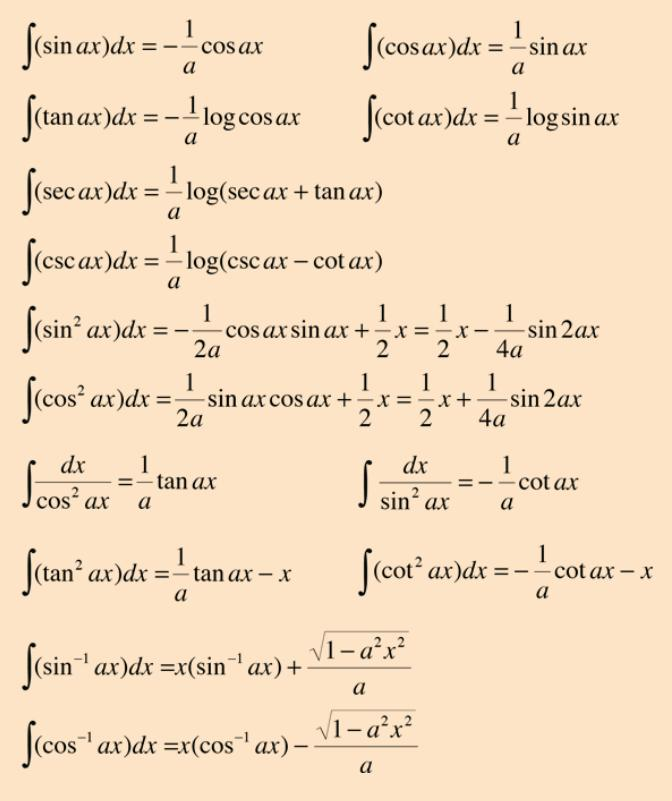
\includegraphics[width = \textwidth]{70}
\end{slika} 


\chapter*{Določeni integral}


\section*{Definicija določenega integrala}
Določeni integral v mejah od $a$ do $ b$ nam pove ploščino lika, ki ga oklepa graf funkcije z abscisno osjo na intervalu $[a,b]$. Definirali smo ga s pomočjo Riemannovih vsot.

\section*{Lastnosti določenega integrala}
Če sta meji enaki, je vrednost integrala enaka 0.
Če damo minus pred integral s tem obrnemo integracijske meje.
Integral vsote je vsota integralov in konstanto lahko nesemo pred integral (enako kot pri nedoločenem).
Integracijsko spremenljivko lahko poljubno označimo.
Integral $a \to b$ kjer $a < c < b$ lahko zapisemo kot vsoto integralov  $a \to c$ in  $c \to b$.

\section*{Izrek o povprečni vrednosti funkcije}
Reče se mu tudi Lagrangeov izrek. V danem odseku funkcije obstaja točka kjer je odvod (nagib) krivulje enak "povprečnemu" odvodu intervala. Izrek se uporablja pri dokazovanju izrekov, ki obravnavajo funkcije na intervalu. 

\[P=\frac{1}{b-a}\int_a^bf(x)dx\]

Izrek o povprečni vrednosti: $m$ je natančna spodnja meja in $M$ natančna zgornja meja integrabilne funkcije $f$ na intervalu $[a,b]$. Potem obstaja tako število $P$, da je $ m< P < M$ in 

\[P=\frac{1}{b-a}\int_a^bf(x)dx\]

Če je funkcija f tudi zvezna na intervalu [a,b], potem obstaja vsaj ena taka točka $\xi \in [a,b]$, da je $f(\xi)=\frac{1}{b-a}\int_a^bf(x)dx$

\section*{Zveza med določenim in nedoločenim integralom}

Med nedoločenim in določenim integralom velja zveza, ki jo imenujemo Newton-Leibnitzova formula ali osnovni izrek integralskega računa:	\\
Določeni integral je razlika nedoločenih integralov na zgornji in spodnji meji. $\int_a^bf(x)dx=F(b)-F(a)$, pri čemer $F'(x)=f(x)$

\section*{Nova spremenljivka in per-partes za določeni integral}
Določeni integral z uvedbo nove spremenljivke $t=f(x)$ se računa na enak način kot nedoločeni, se pa spremenijo meje. Če so bile prejšnje meje $a$ in $b$ so zdaj $f(a$) in $f(b)$
Pri per partes se meje ohranijo
\[\int_a^budv=(uv)|_a^b-\int_a^bvdu\]
 

\section*{Posplošeni integral funkcije}
Uporablja se za integrale neomejenih funkcij ali funkcij na neomejenih intervalih
primer neomejene funkcije $\frac{1}{x}$ v $x=0$
Posplošeni integral za funkcijo neomejeno v točki $b$ na intervalu $[a,c], a<b<c$
 
\[\int_a^cf(x)dx=\lim_{\varepsilon \to 0}\int_a^{b-\varepsilon}f(x)dx+\lim_{\varepsilon \to 0}\int_{b+\varepsilon}^cf(x)dx\]

Posplošeni integral za funkcijo na intervalu od a do neskončno

\[\int_a^\infty	f(x)dx = \lim_{b \to \infty}\int_a^bf(x)dx\] 

\section*{Kartezično, polarno in parametrično podane krivulje}
Kartezično: najbolj pogost zapis. $y=f(x)$\\
Polarno: polarni radij v odvisnosti od kota $r=f(\varphi)$\\
Parametrično: podana z več funkcijami $x=f(t)$ $y=g(t)$

\section*{Ploščina krivočrtnih likov}
\[S=\int_{a}^{b}(f(x)-g(x))dx\]

pri čemer je $f(x)$ zgornja in $g(x)$ spodnja funkcija


\section*{Ploščina izseka polarno podane krivulje}
\[S=\frac{1}{2}\int_{\alpha}^{\beta}(r(\varphi))^2d\varphi\]

\section*{Dolžina krivulje}
\[s=\int_{a}^{b}\sqrt{1+{(f'(x))}^2}dx\]

\section*{Prostornina vrtenine}
\[V=\pi\cdot\int_{a}^{b}{(f(x))}^2dx\]

\section*{Površina vrtenine}
\[ P=2\pi\cdot\int_{a}^{b}f(x)\cdot\sqrt{1+{(f'(x))}^2}dx\]


\end{document}
